\documentclass[aspectratio=169]{beamer}

\usetheme{default}
\usecolortheme{dove}

\setbeamertemplate{navigation symbols}{}
\setbeamertemplate{footline}{%
  \hfill{\large\insertframenumber\,/\,\inserttotalframenumber}\hspace{0.8em}\vspace{0.5em}%
}

\definecolor{popblue}{RGB}{52, 101, 164}
\definecolor{sampred}{RGB}{204, 0, 0}
\definecolor{paramgreen}{RGB}{0, 140, 70}
\definecolor{warnred}{RGB}{180, 40, 40}
\definecolor{orange1}{RGB}{220, 120, 0}
\definecolor{violet1}{RGB}{120, 50, 160}
\definecolor{lightbg}{RGB}{245, 245, 250}

\setbeamercolor{frametitle}{fg=popblue}
\setbeamercolor{title}{fg=popblue}

\usepackage{pgfplots}
\usepackage{tikz}
\usetikzlibrary{shapes, arrows.meta, positioning, calc, decorations.pathreplacing, patterns}
\pgfplotsset{compat=1.18}
\usepackage{amsmath, amssymb}
\usepackage{fontenc}
\usepackage{graphicx}

\title{Lecture 2: Descriptive Statistics}
\subtitle{Center $\cdot$ Spread $\cdot$ Quantiles $\cdot$ Shape $\cdot$ ECDF $\cdot$ Anscombe $\cdot$ Simpson}
\date{}

\begin{document}

% ============================================================
\begin{frame}
\titlepage
\end{frame}

% ============================================================
\begin{frame}
\frametitle{You get a spreadsheet with 10,000 rows\ldots}
\begin{center}
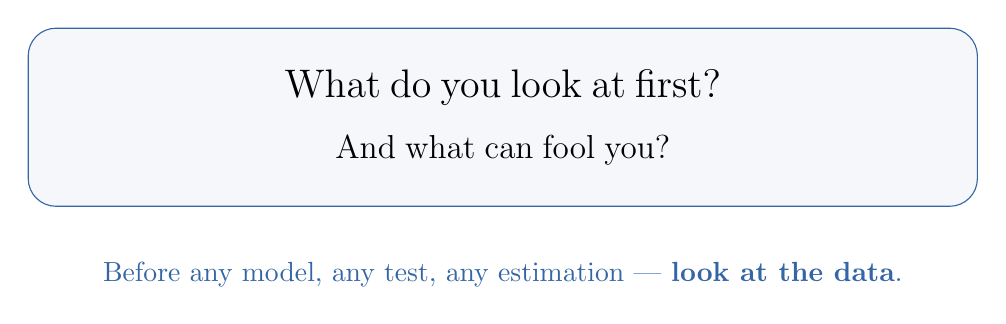
\begin{tikzpicture}
  \node[draw=popblue, fill=popblue!5, rounded corners=10pt, text width=11cm, align=center, inner sep=15pt] {
    {\Large What do you look at first?}\\[10pt]
    {\large And what can fool you?}
  };
  \node[font=\normalsize, text=popblue] at (0, -2) {Before any model, any test, any estimation --- \textbf{look at the data}.};
\end{tikzpicture}
\end{center}
\end{frame}

% ============================================================
\begin{frame}
\frametitle{Goals of Descriptive Statistics}
\begin{center}
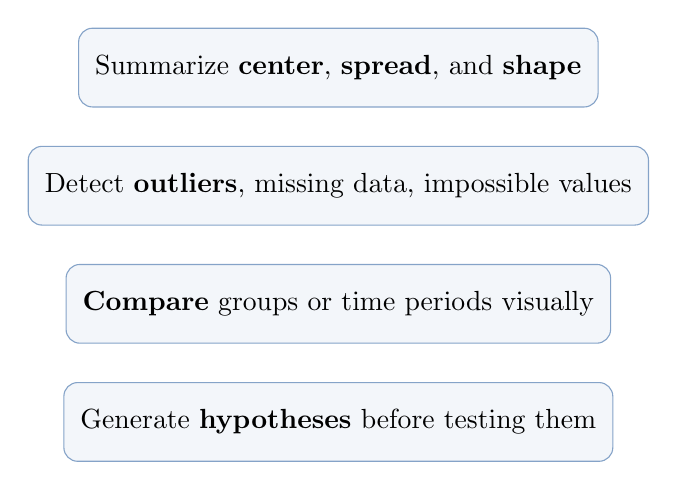
\begin{tikzpicture}[
  gbox/.style={draw=popblue!60, fill=popblue!6, rounded corners=5pt, minimum width=5cm, minimum height=1cm, align=center, font=\normalsize, inner sep=6pt}
]
  \node[gbox] at (0, 2.5) {Summarize \textbf{center}, \textbf{spread}, and \textbf{shape}};
  \node[gbox] at (0, 1) {Detect \textbf{outliers}, missing data, impossible values};
  \node[gbox] at (0, -0.5) {\textbf{Compare} groups or time periods visually};
  \node[gbox] at (0, -2) {Generate \textbf{hypotheses} before testing them};
\end{tikzpicture}
\end{center}
\vspace{0.4cm}
\begin{center}
\small Descriptive $\ne$ inferential: we're describing \textit{this sample}, not yet the population.
\end{center}
\end{frame}

% ============================================================
\section{Measures of Center}

\begin{frame}
\frametitle{Measures of Center}
\begin{center}
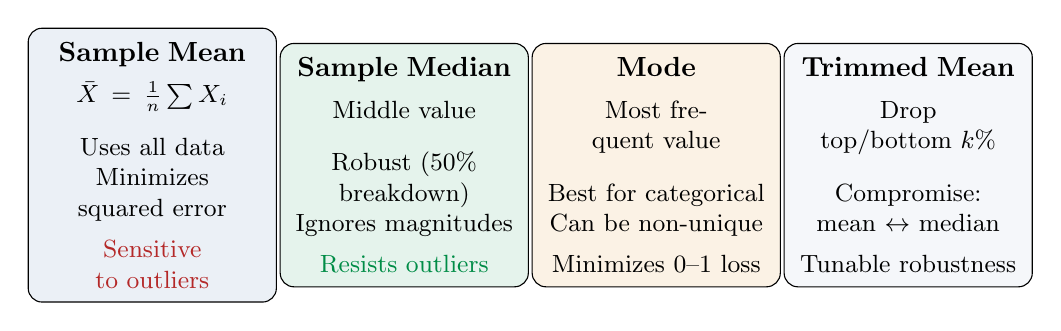
\begin{tikzpicture}[
  mbox/.style={draw, rounded corners=5pt, minimum width=3cm, minimum height=3cm, align=center, text width=2.8cm, inner sep=5pt, font=\small}
]
  \node[mbox, fill=popblue!10] at (-4.8, 0) {
    \textbf{\normalsize Sample Mean}\\[4pt]
    $\bar{X} = \frac{1}{n}\sum X_i$\\[8pt]
    Uses all data\\
    Minimizes squared error\\[4pt]
    \textcolor{warnred}{Sensitive to outliers}
  };
  \node[mbox, fill=paramgreen!10] at (-1.6, 0) {
    \textbf{\normalsize Sample Median}\\[4pt]
    Middle value\\[8pt]
    Robust (50\% breakdown)\\
    Ignores magnitudes\\[4pt]
    \textcolor{paramgreen}{Resists outliers}
  };
  \node[mbox, fill=orange1!10] at (1.6, 0) {
    \textbf{\normalsize Mode}\\[4pt]
    Most frequent value\\[8pt]
    Best for categorical\\
    Can be non-unique\\[4pt]
    Minimizes 0--1 loss
  };
  \node[mbox, fill=popblue!5] at (4.8, 0) {
    \textbf{\normalsize Trimmed Mean}\\[4pt]
    Drop top/bottom $k\%$\\[8pt]
    Compromise:\\
    mean $\leftrightarrow$ median\\[4pt]
    Tunable robustness
  };
\end{tikzpicture}
\end{center}
\end{frame}

% ============================================================
\section{Measures of Spread}

\begin{frame}
\frametitle{Measures of Spread}
\begin{center}
\small
\renewcommand{\arraystretch}{1.5}
\begin{tabular}{llp{5cm}}
  \textbf{Measure} & \textbf{Formula} & \textbf{Properties} \\
  \hline
  Variance $S^2$ & $\frac{1}{n-1}\sum(X_i - \bar{X})^2$ & Uses all data; $n{-}1$ = Bessel's correction (unbiased) \\
  Std Dev $S$ & $\sqrt{S^2}$ & Same units as data \\
  Range & $\max - \min$ & Simple; extremely fragile \\
  IQR & $Q_3 - Q_1$ & Middle 50\%; robust \\
  MAD & $\text{med}\,|X_i - \text{med}|$ & Most robust; companion to median \\
  \hline
\end{tabular}
\end{center}

\vspace{0.3cm}
\begin{center}
\small \textbf{Why $n-1$?} We used up one ``degree of freedom'' estimating $\bar{X}$.\\
This makes $S^2$ \textbf{unbiased}: $\mathbb{E}[S^2] = \sigma^2$.
\end{center}
\end{frame}

\begin{frame}
\frametitle{Robust vs Non-Robust: Visual}
\begin{center}
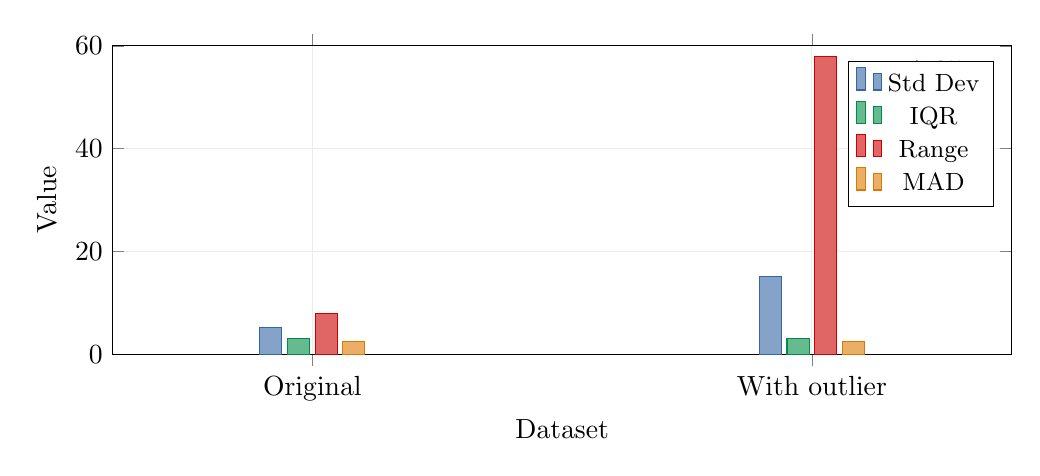
\begin{tikzpicture}
  \begin{axis}[
    width=13cm, height=5.5cm,
    ybar, bar width=8pt,
    xlabel={Dataset},
    ylabel={Value},
    xtick={1,2},
    xticklabels={Original, With outlier},
    ymin=0, ymax=60,
    legend style={at={(0.98,0.95)}, anchor=north east, font=\small},
    grid=major, grid style={gray!15},
    enlarge x limits=0.4,
  ]
    % Original
    \addplot[fill=popblue!60, draw=popblue] coordinates {(1, 5.2) (2, 15.1)};
    \addlegendentry{Std Dev}
    \addplot[fill=paramgreen!60, draw=paramgreen] coordinates {(1, 3.0) (2, 3.0)};
    \addlegendentry{IQR}
    \addplot[fill=sampred!60, draw=sampred] coordinates {(1, 8) (2, 58)};
    \addlegendentry{Range}
    \addplot[fill=orange1!60, draw=orange1] coordinates {(1, 2.5) (2, 2.5)};
    \addlegendentry{MAD}
    \node[font=\small\bfseries, sampred] at (axis cs:2.25, 55) {$\uparrow$ 95};
  \end{axis}
\end{tikzpicture}
\end{center}
\vspace{0.1cm}
\begin{center}
\small One outlier: Range explodes, Std Dev triples. IQR and MAD don't budge.
\end{center}
\end{frame}

% ============================================================
\section{Histograms}

\begin{frame}
\frametitle{How a Histogram Is Built}
\begin{columns}[T]
\begin{column}{0.45\textwidth}
\textbf{Recipe:}
\begin{enumerate}
  \small
  \item Choose \textbf{bins}: equal-width intervals covering the data range
  \item Count observations in each bin
  \item Draw bars --- height $=$ count (or density)
\end{enumerate}

\vspace{0.3cm}
\textbf{Density form:}
$$\text{height} = \frac{\text{count}}{n \times \text{bin width}}$$
so total area $= 1$ (comparable across bin widths).
\end{column}
\begin{column}{0.52\textwidth}
\begin{center}
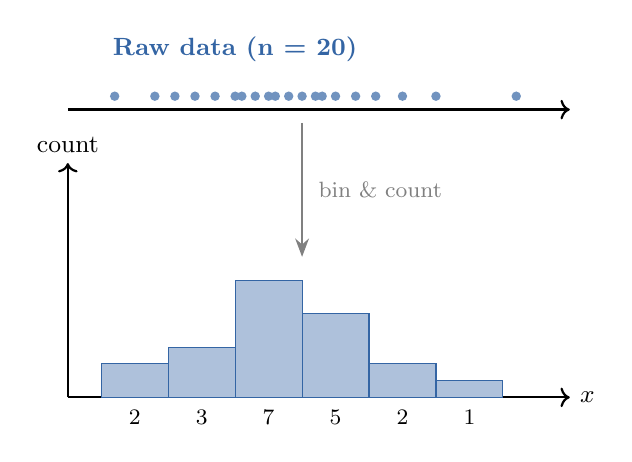
\begin{tikzpicture}[scale=0.85]
  % Raw data points
  \node[font=\small\bfseries, popblue] at (3, 5.2) {Raw data (n = 20)};
  \foreach \x in {1.2, 1.8, 2.1, 2.4, 2.7, 3.0, 3.1, 3.3, 3.5, 3.6, 3.8, 4.0, 4.2, 4.3, 4.5, 4.8, 5.1, 5.5, 6.0, 7.2} {
    \fill[popblue!70] (\x, 4.5) circle (2pt);
  }
  \draw[thick, ->] (0.5, 4.3) -- (8, 4.3);

  % Histogram
  \draw[thick, ->] (0.5, 0) -- (8, 0) node[right, font=\small] {$x$};
  \draw[thick, ->] (0.5, 0) -- (0.5, 3.5) node[above, font=\small] {count};
  % Bins: [1,2), [2,3), [3,4), [4,5), [5,6), [6,7), [7,8)
  \fill[popblue!40, draw=popblue] (1, 0) rectangle (2, 0.5);   % 2
  \fill[popblue!40, draw=popblue] (2, 0) rectangle (3, 0.75);  % 3
  \fill[popblue!40, draw=popblue] (3, 0) rectangle (4, 1.75);  % 7
  \fill[popblue!40, draw=popblue] (4, 0) rectangle (5, 1.25);  % 5
  \fill[popblue!40, draw=popblue] (5, 0) rectangle (6, 0.5);   % 2
  \fill[popblue!40, draw=popblue] (6, 0) rectangle (7, 0.25);  % 1

  % Count labels
  \foreach \x/\c in {1.5/2, 2.5/3, 3.5/7, 4.5/5, 5.5/2, 6.5/1} {
    \node[font=\footnotesize] at (\x, -0.3) {\c};
  }

  % Arrow from data to histogram
  \draw[-{Stealth}, thick, gray] (4, 4.1) -- (4, 2.1);
  \node[font=\footnotesize, gray, right] at (4.1, 3.1) {bin \& count};
\end{tikzpicture}
\end{center}
\end{column}
\end{columns}
\end{frame}

\begin{frame}
\frametitle{Bin Width Matters}
\begin{center}
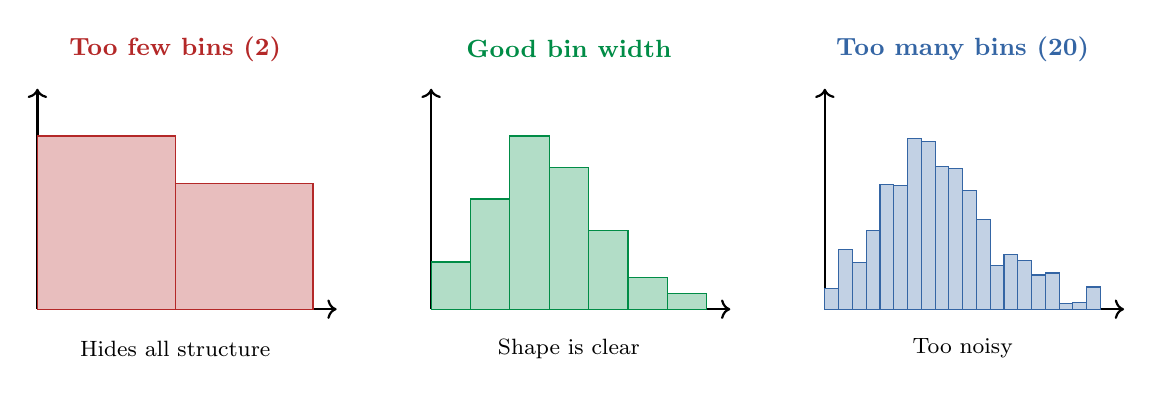
\begin{tikzpicture}
  % Too few bins
  \begin{scope}[xshift=-5cm]
    \node[font=\small\bfseries, warnred] at (1.75, 3.3) {Too few bins (2)};
    \draw[thick, ->] (0, 0) -- (3.8, 0);
    \draw[thick, ->] (0, 0) -- (0, 2.8);
    \fill[warnred!30, draw=warnred] (0, 0) rectangle (1.75, 2.2);
    \fill[warnred!30, draw=warnred] (1.75, 0) rectangle (3.5, 1.6);
    \node[font=\footnotesize] at (1.75, -0.5) {Hides all structure};
  \end{scope}

  % Just right
  \begin{scope}[xshift=0cm]
    \node[font=\small\bfseries, paramgreen] at (1.75, 3.3) {Good bin width};
    \draw[thick, ->] (0, 0) -- (3.8, 0);
    \draw[thick, ->] (0, 0) -- (0, 2.8);
    \fill[paramgreen!30, draw=paramgreen] (0, 0) rectangle (0.5, 0.6);
    \fill[paramgreen!30, draw=paramgreen] (0.5, 0) rectangle (1.0, 1.4);
    \fill[paramgreen!30, draw=paramgreen] (1.0, 0) rectangle (1.5, 2.2);
    \fill[paramgreen!30, draw=paramgreen] (1.5, 0) rectangle (2.0, 1.8);
    \fill[paramgreen!30, draw=paramgreen] (2.0, 0) rectangle (2.5, 1.0);
    \fill[paramgreen!30, draw=paramgreen] (2.5, 0) rectangle (3.0, 0.4);
    \fill[paramgreen!30, draw=paramgreen] (3.0, 0) rectangle (3.5, 0.2);
    \node[font=\footnotesize] at (1.75, -0.5) {Shape is clear};
  \end{scope}

  % Too many bins
  \begin{scope}[xshift=5cm]
    \node[font=\small\bfseries, popblue] at (1.75, 3.3) {Too many bins (20)};
    \draw[thick, ->] (0, 0) -- (3.8, 0);
    \draw[thick, ->] (0, 0) -- (0, 2.8);
    \foreach \i in {0,...,19} {
      \pgfmathsetmacro{\h}{0.2 + 2.0*exp(-(\i-7)*(\i-7)/18) + 0.3*rand}
      \pgfmathsetmacro{\xl}{0.175*\i}
      \pgfmathsetmacro{\xr}{0.175*(\i+1)}
      \fill[popblue!30, draw=popblue] (\xl, 0) rectangle (\xr, \h);
    }
    \node[font=\footnotesize] at (1.75, -0.5) {Too noisy};
  \end{scope}
\end{tikzpicture}
\end{center}

\vspace{0.3cm}
\begin{center}
\small \textbf{Common rules:} Sturges ($k = 1 + \log_2 n$), Freedman--Diaconis ($h = 2 \cdot \text{IQR} \cdot n^{-1/3}$).\\
In practice: try several and look.
\end{center}
\end{frame}

% ============================================================
\section{Quantiles and Boxplots}

\begin{frame}
\frametitle{Quantiles and Percentiles}
\begin{center}
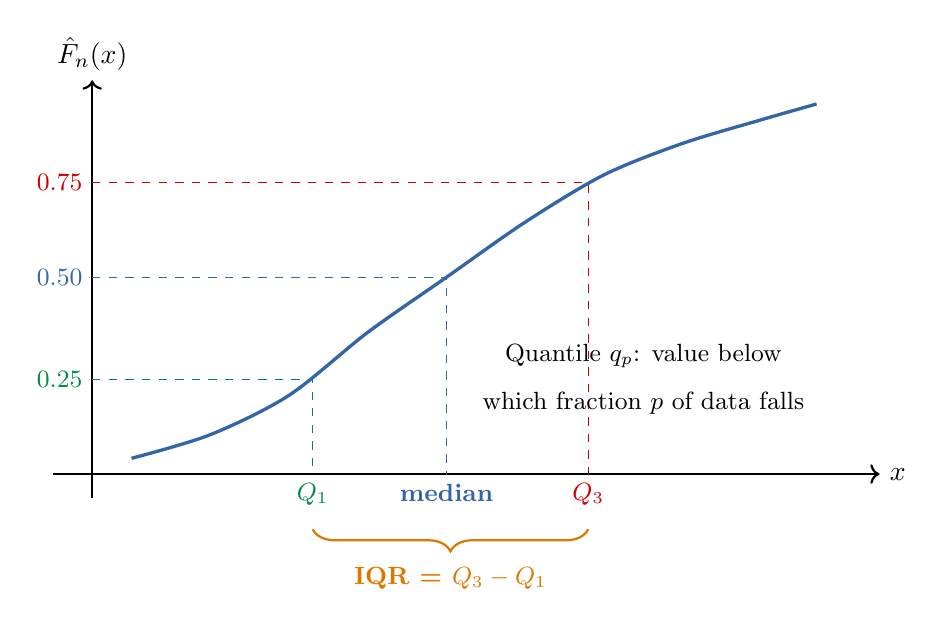
\begin{tikzpicture}
  % CDF-like curve
  \draw[thick, ->] (-0.5, 0) -- (10, 0) node[right] {$x$};
  \draw[thick, ->] (0, -0.3) -- (0, 5) node[above] {$\hat{F}_n(x)$};

  % S-curve
  \draw[very thick, popblue, smooth] plot coordinates {
    (0.5, 0.2) (1.5, 0.5) (2.5, 1.0) (3.5, 1.8) (4.5, 2.5)
    (5.5, 3.2) (6.5, 3.8) (7.5, 4.2) (8.5, 4.5) (9.2, 4.7)
  };

  % Horizontal lines at 25%, 50%, 75%
  \draw[dashed, paramgreen] (0, 1.2) -- (2.8, 1.2) -- (2.8, 0);
  \node[left, font=\small, paramgreen] at (0, 1.2) {0.25};
  \node[below, font=\small\bfseries, paramgreen] at (2.8, 0) {$Q_1$};

  \draw[dashed, popblue] (0, 2.5) -- (4.5, 2.5) -- (4.5, 0);
  \node[left, font=\small, popblue] at (0, 2.5) {0.50};
  \node[below, font=\small\bfseries, popblue] at (4.5, 0) {median};

  \draw[dashed, sampred] (0, 3.7) -- (6.3, 3.7) -- (6.3, 0);
  \node[left, font=\small, sampred] at (0, 3.7) {0.75};
  \node[below, font=\small\bfseries, sampred] at (6.3, 0) {$Q_3$};

  % IQR brace
  \draw[decorate, decoration={brace, amplitude=8pt, mirror}, thick, orange1]
    (2.8, -0.7) -- (6.3, -0.7) node[midway, below=10pt, font=\small\bfseries, orange1] {IQR = $Q_3 - Q_1$};

  % Labels
  \node[font=\small] at (7, 1.5) {Quantile $q_p$: value below};
  \node[font=\small] at (7, 0.9) {which fraction $p$ of data falls};
\end{tikzpicture}
\end{center}
\end{frame}

\begin{frame}
\frametitle{Boxplot Anatomy}
\begin{center}
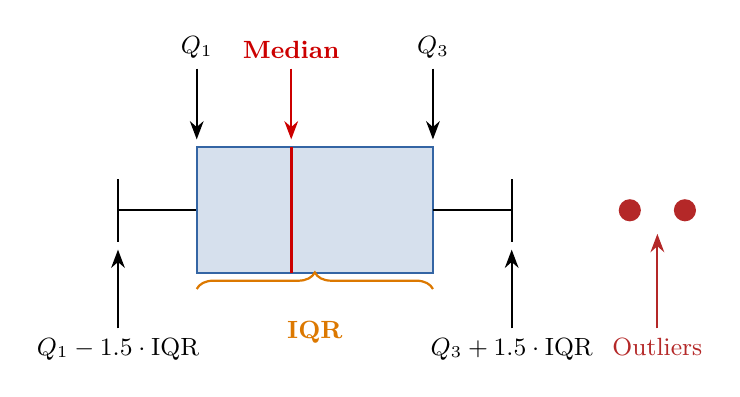
\begin{tikzpicture}
  % The boxplot (horizontal)
  \draw[thick] (2, 0) -- (7, 0); % lower whisker
  \draw[thick] (2, -0.4) -- (2, 0.4); % lower whisker cap
  \fill[popblue!20, draw=popblue, thick] (3, -0.8) rectangle (6, 0.8); % box
  \draw[very thick, sampred] (4.2, -0.8) -- (4.2, 0.8); % median
  \draw[thick] (7, -0.4) -- (7, 0.4); % upper whisker cap
  \draw[thick] (6, 0) -- (7, 0); % upper whisker

  % Outlier dots
  \fill[warnred] (8.5, 0) circle (4pt);
  \fill[warnred] (9.2, 0) circle (4pt);

  % Labels with arrows
  \draw[-{Stealth}, thick] (2, -1.5) -- (2, -0.5);
  \node[font=\small, below] at (2, -1.5) {$Q_1 - 1.5 \cdot\text{IQR}$};

  \draw[-{Stealth}, thick] (3, 1.8) -- (3, 0.9);
  \node[font=\small, above] at (3, 1.8) {$Q_1$};

  \draw[-{Stealth}, thick, sampred] (4.2, 1.8) -- (4.2, 0.9);
  \node[font=\small\bfseries, above, sampred] at (4.2, 1.8) {Median};

  \draw[-{Stealth}, thick] (6, 1.8) -- (6, 0.9);
  \node[font=\small, above] at (6, 1.8) {$Q_3$};

  \draw[-{Stealth}, thick] (7, -1.5) -- (7, -0.5);
  \node[font=\small, below] at (7, -1.5) {$Q_3 + 1.5 \cdot\text{IQR}$};

  \draw[-{Stealth}, thick, warnred] (8.85, -1.5) -- (8.85, -0.3);
  \node[font=\small, below, warnred] at (8.85, -1.5) {Outliers};

  % IQR brace
  \draw[decorate, decoration={brace, amplitude=6pt}, thick, orange1]
    (3, -1.0) -- (6, -1.0) node[midway, below=8pt, font=\small\bfseries, orange1] {IQR};
\end{tikzpicture}
\end{center}

\vspace{0.15cm}
\begin{center}
\small \textbf{Five-number summary:} $\min, \; Q_1, \; \text{median}, \; Q_3, \; \max$ --- the boxplot visualizes exactly this.
\end{center}
\vspace{0.05cm}
\begin{columns}
\begin{column}{0.48\textwidth}
\textbf{Strengths:}
\begin{itemize}
  \small
  \item Compact group comparison
  \item Shows center, spread, outliers
\end{itemize}
\end{column}
\begin{column}{0.48\textwidth}
\textbf{Weakness:}
\begin{itemize}
  \small
  \item Hides multimodality!
  \item Pair with histogram or violin
\end{itemize}
\end{column}
\end{columns}
\end{frame}

\begin{frame}
\frametitle{Boxplot Hides Bimodality}
\begin{center}
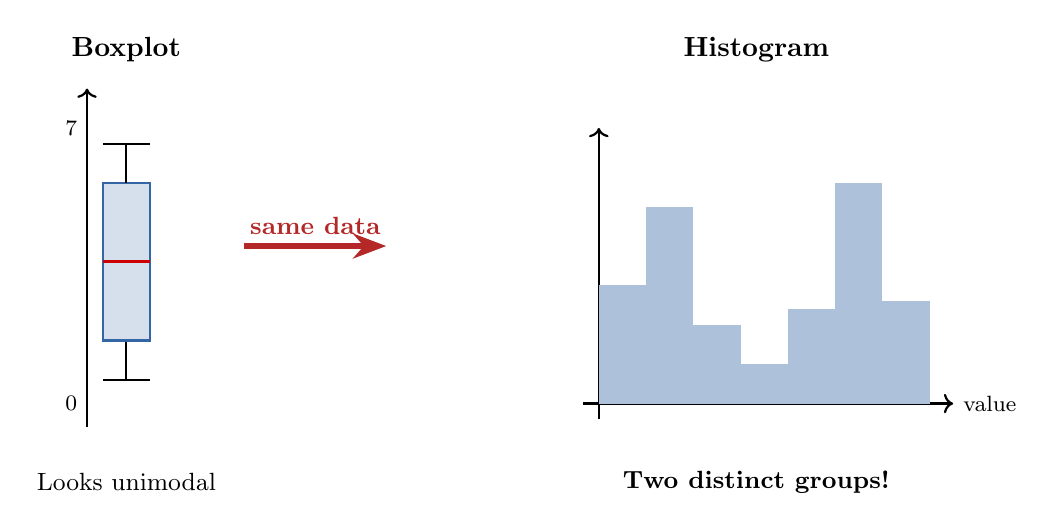
\begin{tikzpicture}
  % Left: vertical boxplot
  \begin{scope}[xshift=-4cm]
    \node[font=\bfseries] at (2, 4.5) {Boxplot};
    \draw[thick, ->] (1.5, -0.3) -- (1.5, 4);
    \node[left, font=\footnotesize] at (1.5, 0) {0};
    \node[left, font=\footnotesize] at (1.5, 3.5) {7};
    % Vertical boxplot
    \draw[thick] (2, 0.3) -- (2, 0.8); % lower whisker
    \draw[thick] (1.7, 0.3) -- (2.3, 0.3); % lower cap
    \fill[popblue!20, draw=popblue, thick] (1.7, 0.8) rectangle (2.3, 2.8); % box
    \draw[very thick, sampred] (1.7, 1.8) -- (2.3, 1.8); % median
    \draw[thick] (2, 2.8) -- (2, 3.3); % upper whisker
    \draw[thick] (1.7, 3.3) -- (2.3, 3.3); % upper cap
    \node[font=\small] at (2, -1) {Looks unimodal};
  \end{scope}

  % Right: the histogram (bimodal, vertical bars matching same y-axis)
  \begin{scope}[xshift=4cm]
    \node[font=\bfseries] at (2, 4.5) {Histogram};
    \draw[thick, ->] (-0.2, 0) -- (4.5, 0) node[right, font=\footnotesize] {value};
    \draw[thick, ->] (0, -0.2) -- (0, 3.5);
    \fill[popblue!40] (0, 0) rectangle (0.6, 1.5);
    \fill[popblue!40] (0.6, 0) rectangle (1.2, 2.5);
    \fill[popblue!40] (1.2, 0) rectangle (1.8, 1.0);
    \fill[popblue!40] (1.8, 0) rectangle (2.4, 0.5);
    \fill[popblue!40] (2.4, 0) rectangle (3.0, 1.2);
    \fill[popblue!40] (3.0, 0) rectangle (3.6, 2.8);
    \fill[popblue!40] (3.6, 0) rectangle (4.2, 1.3);
    \node[font=\small] at (2, -1) {\textbf{Two distinct groups!}};
  \end{scope}

  % Arrow
  \draw[-{Stealth}, very thick, warnred, line width=2pt] (-0.5, 2) -- (1.3, 2)
    node[midway, above, font=\small\bfseries, warnred] {same data};
\end{tikzpicture}
\end{center}

\vspace{0.3cm}
\begin{center}
\fcolorbox{warnred}{warnred!5}{\parbox{10cm}{\centering\small Always pair boxplots with histograms or violin plots.}}
\end{center}
\end{frame}

% ============================================================
\section{Shape: Skewness and Kurtosis}

\begin{frame}
\frametitle{Skewness: Measuring Asymmetry}
\begin{center}
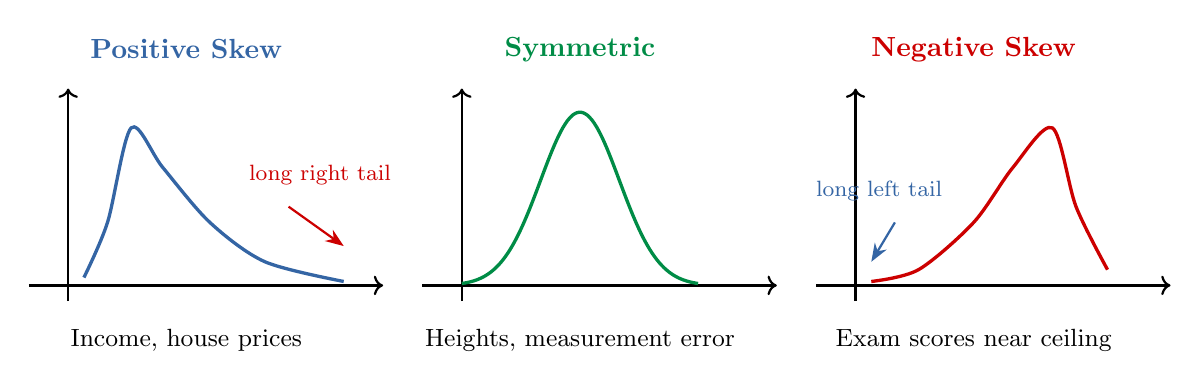
\begin{tikzpicture}
  % Positive skew
  \begin{scope}[xshift=-5cm]
    \node[font=\bfseries, popblue] at (1.5, 3) {Positive Skew};
    \draw[thick, ->] (-0.5, 0) -- (4, 0);
    \draw[thick, ->] (0, -0.2) -- (0, 2.5);
    \draw[very thick, popblue, smooth] plot coordinates {
      (0.2, 0.1) (0.5, 0.8) (0.8, 2.0) (1.2, 1.5) (1.8, 0.8) (2.5, 0.3) (3.5, 0.05)
    };
    \node[font=\small] at (1.5, -0.7) {Income, house prices};
    \draw[-{Stealth}, thick, sampred] (2.8, 1) -- (3.5, 0.5);
    \node[font=\footnotesize, sampred] at (3.2, 1.4) {long right tail};
  \end{scope}

  % Symmetric
  \begin{scope}[xshift=0cm]
    \node[font=\bfseries, paramgreen] at (1.5, 3) {Symmetric};
    \draw[thick, ->] (-0.5, 0) -- (4, 0);
    \draw[thick, ->] (0, -0.2) -- (0, 2.5);
    \draw[very thick, paramgreen, smooth, domain=0:3, samples=50] plot (\x, {2.2*exp(-(\x-1.5)*(\x-1.5)/0.5)});
    \node[font=\small] at (1.5, -0.7) {Heights, measurement error};
  \end{scope}

  % Negative skew
  \begin{scope}[xshift=5cm]
    \node[font=\bfseries, sampred] at (1.5, 3) {Negative Skew};
    \draw[thick, ->] (-0.5, 0) -- (4, 0);
    \draw[thick, ->] (0, -0.2) -- (0, 2.5);
    \draw[very thick, sampred, smooth] plot coordinates {
      (0.2, 0.05) (0.8, 0.2) (1.5, 0.8) (2.0, 1.5) (2.5, 2.0) (2.8, 1.0) (3.2, 0.2)
    };
    \node[font=\small] at (1.5, -0.7) {Exam scores near ceiling};
    \draw[-{Stealth}, thick, popblue] (0.5, 0.8) -- (0.2, 0.3);
    \node[font=\footnotesize, popblue] at (0.3, 1.2) {long left tail};
  \end{scope}
\end{tikzpicture}
\end{center}

\vspace{0.2cm}
$$\text{Skewness} = \frac{1}{n}\sum_{i=1}^n\left(\frac{X_i - \bar{X}}{S}\right)^3$$
\end{frame}

\begin{frame}
\frametitle{Kurtosis: Tail Heaviness}
\begin{center}
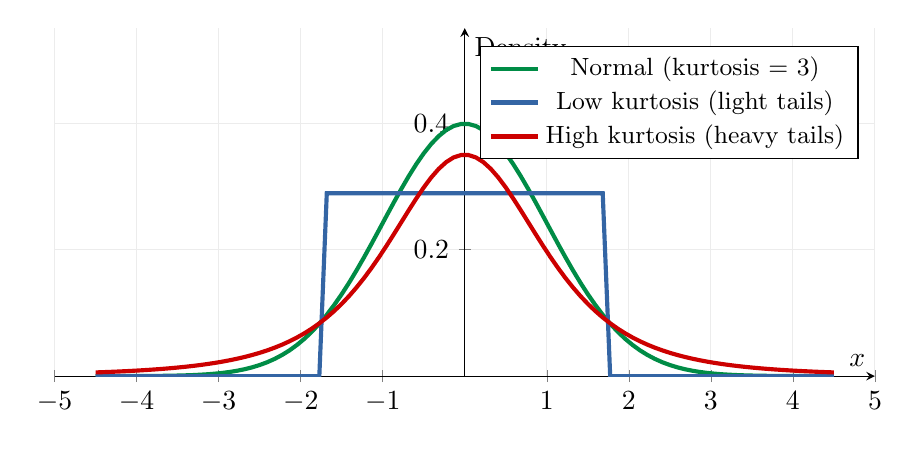
\begin{tikzpicture}
  \begin{axis}[
    width=12cm, height=6cm,
    xlabel={$x$},
    ylabel={Density},
    xmin=-5, xmax=5,
    ymin=0, ymax=0.55,
    axis lines=middle,
    legend style={at={(0.98,0.95)}, anchor=north east, font=\small},
    grid=major, grid style={gray!15},
    every axis plot/.append style={line width=1.5pt, samples=100}
  ]
    % Normal (kurtosis = 3)
    \addplot[paramgreen, domain=-4.5:4.5] {exp(-x^2/2) / sqrt(2*pi)};
    \addlegendentry{Normal (kurtosis = 3)}

    % Low kurtosis (uniform-ish)
    \addplot[popblue, domain=-4.5:4.5] {(abs(x) < 1.73) * 0.289};
    \addlegendentry{Low kurtosis (light tails)}

    % High kurtosis (t-distribution like)
    \addplot[sampred, domain=-4.5:4.5] {0.35 / (1 + x^2/3)^2};
    \addlegendentry{High kurtosis (heavy tails)}
  \end{axis}
\end{tikzpicture}
\end{center}
\vspace{-0.1cm}
$$\text{Kurtosis} = \frac{1}{n}\sum_{i=1}^n\left(\frac{X_i - \bar{X}}{S}\right)^4 \qquad \text{Excess kurtosis} = \text{Kurt} - 3$$

\vspace{-0.2cm}
\begin{center}
\small Normal has kurtosis $= 3$ (excess $= 0$). Most software reports \textbf{excess kurtosis}.\\
\small Financial returns have high kurtosis --- assuming normality underestimates risk.
\end{center}
\end{frame}

% ============================================================
\section{The Empirical CDF}

\begin{frame}
\frametitle{The Empirical CDF}

$$\hat{F}_n(t) = \frac{1}{n}\#\{X_i \le t\} = \frac{\text{number of observations} \le t}{n}$$

\begin{center}
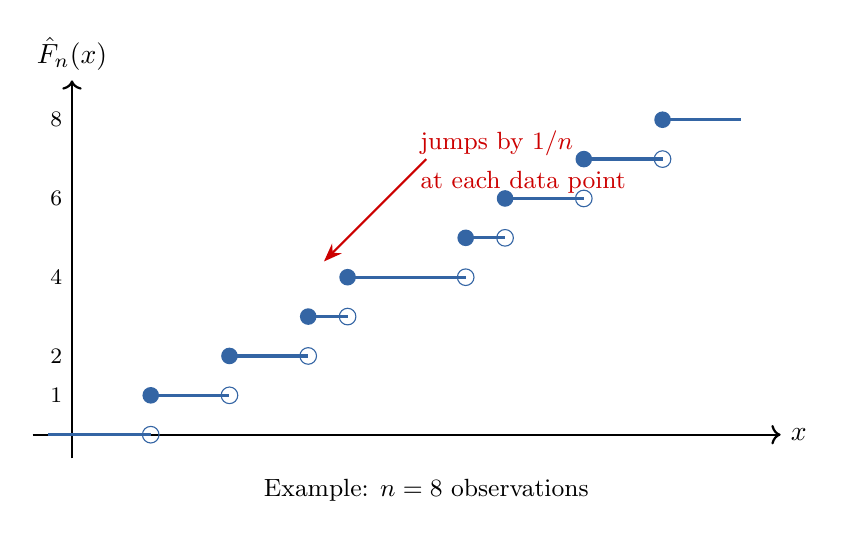
\begin{tikzpicture}
  \draw[thick, ->] (-0.5, 0) -- (9, 0) node[right] {$x$};
  \draw[thick, ->] (0, -0.3) -- (0, 4.5) node[above] {$\hat{F}_n(x)$};

  % Step function (n=8 example)
  \draw[very thick, popblue]
    (-0.3, 0) -- (1, 0)
    (1, 0.5) -- (2, 0.5)
    (2, 1.0) -- (3, 1.0)
    (3, 1.5) -- (3.5, 1.5)
    (3.5, 2.0) -- (5, 2.0)
    (5, 2.5) -- (5.5, 2.5)
    (5.5, 3.0) -- (6.5, 3.0)
    (6.5, 3.5) -- (7.5, 3.5)
    (7.5, 4.0) -- (8.5, 4.0);

  % Jump dots
  \foreach \x/\y in {1/0.5, 2/1.0, 3/1.5, 3.5/2.0, 5/2.5, 5.5/3.0, 6.5/3.5, 7.5/4.0} {
    \fill[popblue] (\x, \y) circle (3pt);
    \draw[popblue] (\x, \y-0.5) circle (3pt);
  }

  % Y-axis labels
  \foreach \y/\lab in {0.5/1/8, 1.0/2/8, 2.0/4/8, 3.0/6/8, 4.0/8/8} {
    \node[left, font=\footnotesize] at (0, \y) {$\lab$};
  }

  % Annotation
  \draw[-{Stealth}, thick, sampred] (4.5, 3.5) -- (3.2, 2.2);
  \node[font=\small, sampred, right] at (4.3, 3.7) {jumps by $1/n$};
  \node[font=\small, sampred, right] at (4.3, 3.2) {at each data point};

  % n label
  \node[font=\small] at (4.5, -0.7) {Example: $n = 8$ observations};
\end{tikzpicture}
\end{center}
\end{frame}

\begin{frame}
\frametitle{ECDF: Why It's Powerful}
\begin{center}
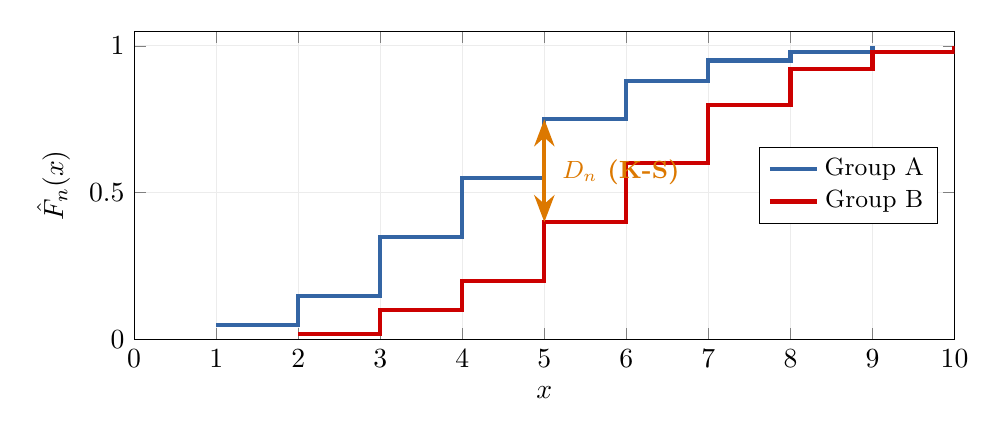
\begin{tikzpicture}
  \begin{axis}[
    width=12cm, height=5.5cm,
    xlabel={$x$},
    ylabel={$\hat{F}_n(x)$},
    xmin=0, xmax=10,
    ymin=0, ymax=1.05,
    legend style={at={(0.98,0.5)}, anchor=east, font=\small},
    grid=major, grid style={gray!15},
    every axis plot/.append style={line width=1.5pt}
  ]
    % Group A ECDF
    \addplot[popblue, const plot] coordinates {
      (1, 0.05) (2, 0.15) (3, 0.35) (4, 0.55) (5, 0.75) (6, 0.88) (7, 0.95) (8, 0.98) (9, 1.0)
    };
    \addlegendentry{Group A}

    % Group B ECDF (shifted right)
    \addplot[sampred, const plot] coordinates {
      (2, 0.02) (3, 0.10) (4, 0.20) (5, 0.40) (6, 0.60) (7, 0.80) (8, 0.92) (9, 0.98) (10, 1.0)
    };
    \addlegendentry{Group B}

    % KS distance
    \draw[{Stealth}-{Stealth}, thick, orange1, line width=1.5pt] (axis cs:5, 0.40) -- (axis cs:5, 0.75);
    \node[font=\small\bfseries, orange1, right] at (axis cs:5.1, 0.57) {$D_n$ (K-S)};
  \end{axis}
\end{tikzpicture}
\end{center}

\begin{itemize}
  \small
  \item No bin-width choice (unlike histograms) --- the ECDF is \textbf{parameter-free}
  \item Biggest gap = \textbf{Kolmogorov--Smirnov statistic} $D_n$
  \item Glivenko--Cantelli: $\hat{F}_n \to F$ uniformly as $n \to \infty$
\end{itemize}
\end{frame}

\begin{frame}
\frametitle{Choosing the Right Plot}
\begin{center}
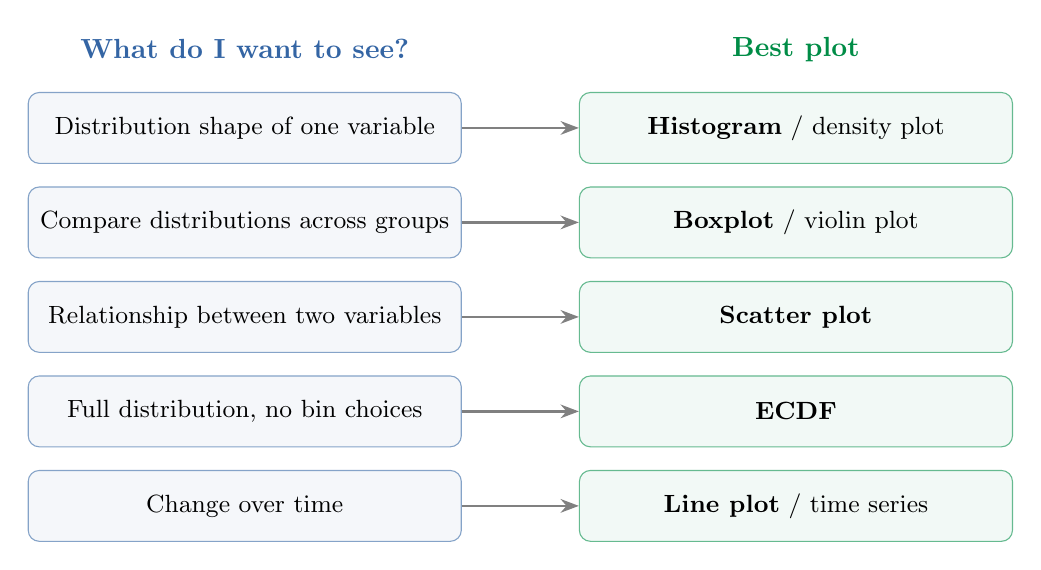
\begin{tikzpicture}[
  qbox/.style={draw=popblue!60, fill=popblue!5, rounded corners=4pt, minimum width=5.5cm, minimum height=0.9cm, align=center, font=\small, inner sep=4pt},
  abox/.style={draw=paramgreen!60, fill=paramgreen!5, rounded corners=4pt, minimum width=5.5cm, minimum height=0.9cm, align=center, font=\small, inner sep=4pt}
]
  % Questions → Plots
  \node[font=\bfseries, popblue] at (-3.5, 3.5) {What do I want to see?};
  \node[font=\bfseries, paramgreen] at (3.5, 3.5) {Best plot};

  \node[qbox] (q1) at (-3.5, 2.5) {Distribution shape of one variable};
  \node[abox] (a1) at (3.5, 2.5) {\textbf{Histogram} / density plot};
  \draw[-{Stealth}, thick, gray] (q1) -- (a1);

  \node[qbox] (q2) at (-3.5, 1.3) {Compare distributions across groups};
  \node[abox] (a2) at (3.5, 1.3) {\textbf{Boxplot} / violin plot};
  \draw[-{Stealth}, thick, gray] (q2) -- (a2);

  \node[qbox] (q3) at (-3.5, 0.1) {Relationship between two variables};
  \node[abox] (a3) at (3.5, 0.1) {\textbf{Scatter plot}};
  \draw[-{Stealth}, thick, gray] (q3) -- (a3);

  \node[qbox] (q4) at (-3.5, -1.1) {Full distribution, no bin choices};
  \node[abox] (a4) at (3.5, -1.1) {\textbf{ECDF}};
  \draw[-{Stealth}, thick, gray] (q4) -- (a4);

  \node[qbox] (q5) at (-3.5, -2.3) {Change over time};
  \node[abox] (a5) at (3.5, -2.3) {\textbf{Line plot} / time series};
  \draw[-{Stealth}, thick, gray] (q5) -- (a5);
\end{tikzpicture}
\end{center}
\vspace{0.1cm}
\begin{center}
\small \textbf{Rule of thumb:} always start with a histogram + scatter plot matrix. Then refine.
\end{center}
\end{frame}

% ============================================================
\section{Summary Statistics Can Lie}

\begin{frame}
\frametitle{Anscombe's Quartet (1973)}
\begin{center}
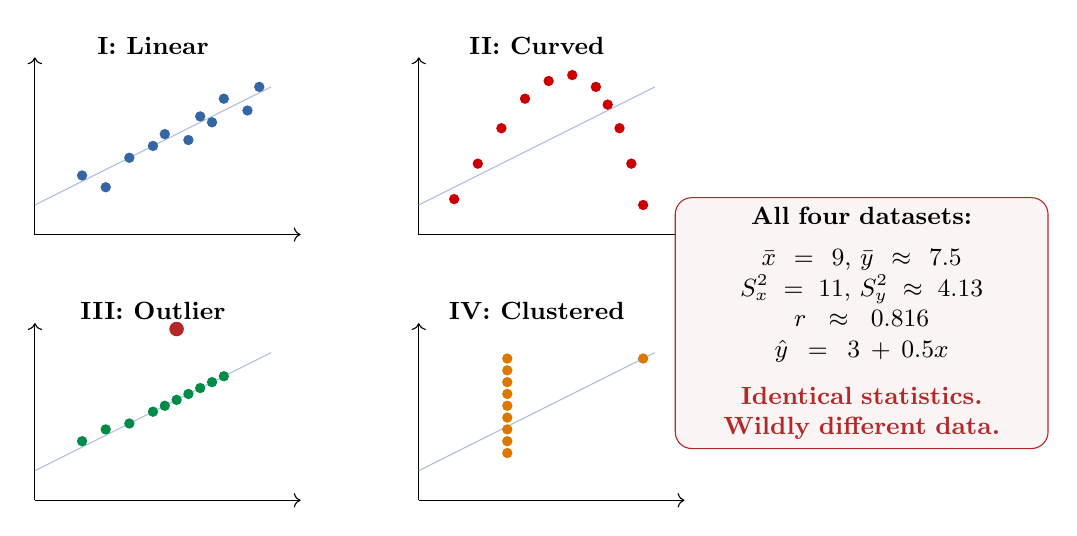
\begin{tikzpicture}[scale=0.75]
  % All four have same: mean x=9, mean y=7.5, var x=11, var y=4.13, corr=0.816, regression: y=3+0.5x

  % Dataset I - linear
  \begin{scope}[xshift=-5.5cm, yshift=2.5cm]
    \node[font=\small\bfseries] at (2, 3.2) {I: Linear};
    \draw[->] (0,0) -- (4.5, 0); \draw[->] (0,0) -- (0, 3);
    \draw[thin, popblue!40] (0, 0.5) -- (4, 2.5);
    \foreach \x/\y in {0.8/1.0, 1.2/0.8, 1.6/1.3, 2.0/1.5, 2.2/1.7, 2.6/1.6, 2.8/2.0, 3.0/1.9, 3.2/2.3, 3.6/2.1, 3.8/2.5} {
      \fill[popblue] (\x, \y) circle (2.5pt);
    }
  \end{scope}

  % Dataset II - curved
  \begin{scope}[xshift=1cm, yshift=2.5cm]
    \node[font=\small\bfseries] at (2, 3.2) {II: Curved};
    \draw[->] (0,0) -- (4.5, 0); \draw[->] (0,0) -- (0, 3);
    \draw[thin, popblue!40] (0, 0.5) -- (4, 2.5);
    \foreach \x/\y in {0.6/0.6, 1.0/1.2, 1.4/1.8, 1.8/2.3, 2.2/2.6, 2.6/2.7, 3.0/2.5, 3.2/2.2, 3.4/1.8, 3.6/1.2, 3.8/0.5} {
      \fill[sampred] (\x, \y) circle (2.5pt);
    }
  \end{scope}

  % Dataset III - outlier
  \begin{scope}[xshift=-5.5cm, yshift=-2cm]
    \node[font=\small\bfseries] at (2, 3.2) {III: Outlier};
    \draw[->] (0,0) -- (4.5, 0); \draw[->] (0,0) -- (0, 3);
    \draw[thin, popblue!40] (0, 0.5) -- (4, 2.5);
    \foreach \x/\y in {0.8/1.0, 1.2/1.2, 1.6/1.3, 2.0/1.5, 2.2/1.6, 2.4/1.7, 2.6/1.8, 2.8/1.9, 3.0/2.0, 3.2/2.1} {
      \fill[paramgreen] (\x, \y) circle (2.5pt);
    }
    \fill[warnred] (2.4, 2.9) circle (3.5pt); % outlier
  \end{scope}

  % Dataset IV - clustered + extreme
  \begin{scope}[xshift=1cm, yshift=-2cm]
    \node[font=\small\bfseries] at (2, 3.2) {IV: Clustered};
    \draw[->] (0,0) -- (4.5, 0); \draw[->] (0,0) -- (0, 3);
    \draw[thin, popblue!40] (0, 0.5) -- (4, 2.5);
    \foreach \y in {0.8, 1.0, 1.2, 1.4, 1.6, 1.8, 2.0, 2.2, 2.4} {
      \fill[orange1] (1.5, \y) circle (2.5pt);
    }
    \fill[orange1] (3.8, 2.4) circle (2.5pt); % extreme x
  \end{scope}

  % Common stats box
  \node[draw=warnred, fill=warnred!5, rounded corners=6pt, text width=4.5cm, align=center, font=\small] at (8.5, 1) {
    \textbf{All four datasets:}\\[4pt]
    $\bar{x} = 9$, $\bar{y} \approx 7.5$\\
    $S_x^2 = 11$, $S_y^2 \approx 4.13$\\
    $r \approx 0.816$\\
    $\hat{y} = 3 + 0.5x$\\[6pt]
    \textcolor{warnred}{\textbf{Identical statistics.}}\\
    \textcolor{warnred}{\textbf{Wildly different data.}}
  };
\end{tikzpicture}
\end{center}
\end{frame}

\begin{frame}
\frametitle{The Datasaurus Dozen (2017)}
\begin{columns}[c]
\begin{column}{0.55\textwidth}
  \begin{center}
    \includegraphics[width=\columnwidth]{../../assets/dinozavrik.png}
  \end{center}
\end{column}
\begin{column}{0.42\textwidth}
  \textbf{13 datasets}, all with:
  \begin{itemize}
    \item Same $\bar{x}$, $\bar{y}$
    \item Same $S_x$, $S_y$
    \item Same correlation $r$
  \end{itemize}

  \vspace{0.4cm}
  Yet shapes include a \textbf{dinosaur}, a star, parallel lines, a circle\ldots

  \vspace{0.4cm}
  \fcolorbox{warnred}{warnred!5}{\parbox{3.8cm}{\centering\small\textbf{Never trust summary\\statistics alone.\\Always plot your data.}}}
\end{column}
\end{columns}
\end{frame}

\begin{frame}
\frametitle{Simpson's Paradox}
\begin{center}
  \includegraphics[width=\columnwidth, height=6.5cm, keepaspectratio]{../../assets/simpson_lines.png}
\end{center}
\vspace{0.1cm}
\begin{center}
\small Each colored group trends \textbf{down}, yet the aggregate trend goes \textbf{up}.\\
How? The groups have \textbf{different sizes and positions}.
\end{center}
\end{frame}

\begin{frame}
\frametitle{Simpson's Paradox: UC Berkeley Admissions (1973)}

\vspace{-0.1cm}
\begin{center}
\small 12{,}763 applicants to UC Berkeley graduate programs.
\end{center}
\vspace{0.1cm}

\begin{columns}[T]
\begin{column}{0.48\textwidth}
\begin{center}
\textbf{\textcolor{sampred}{Aggregate data:}}

\vspace{0.2cm}
\renewcommand{\arraystretch}{1.3}
\begin{tabular}{lcc}
  & \textbf{Applied} & \textbf{Admitted} \\
  \hline
  Men & 8{,}442 & 44\% \\
  Women & 4{,}321 & 35\% \\
  \hline
\end{tabular}

\vspace{0.3cm}
\fcolorbox{sampred}{sampred!5}{\parbox{4.5cm}{\centering\small 9 percentage points gap!\\Lawsuit filed for gender bias.}}
\end{center}
\end{column}
\begin{column}{0.48\textwidth}
\begin{center}
\textbf{\textcolor{paramgreen}{By department:}}

\vspace{0.2cm}
\renewcommand{\arraystretch}{1.3}
\small
\begin{tabular}{lccc}
  & \textbf{Rate} & \textbf{Women} & \textbf{Men} \\
  \hline
  Dept A & easy & 82\% & 62\% \\
  Dept B & easy & 68\% & 63\% \\
  Dept C & hard & 34\% & 35\% \\
  Dept D & hard & 7\% & 6\% \\
  \hline
\end{tabular}

\vspace{0.3cm}
\fcolorbox{paramgreen}{paramgreen!5}{\parbox{4.5cm}{\centering\small Women admitted at equal or\\
\textbf{higher} rates in each dept!}}
\end{center}
\end{column}
\end{columns}

\vspace{0.3cm}
\begin{center}
\textbf{\textcolor{warnred}{How is this possible?}}
\end{center}
\end{frame}

\begin{frame}
\frametitle{Simpson's Paradox: Why It Happens}

\vspace{-0.1cm}
\begin{center}
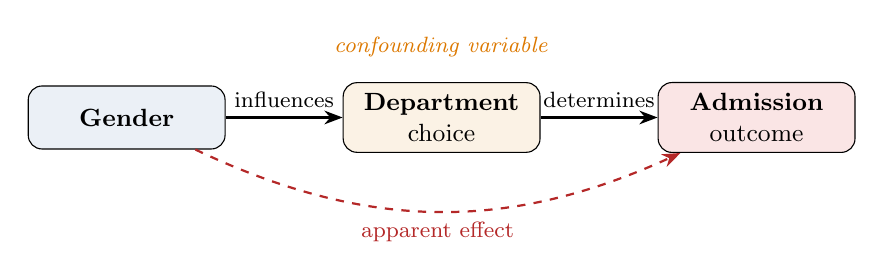
\begin{tikzpicture}[
  box/.style={draw, rounded corners=5pt, minimum width=2.5cm, minimum height=0.8cm, align=center, font=\small, inner sep=4pt}
]
  \node[box, fill=popblue!10] (gender) at (-4, 0) {\textbf{Gender}};
  \node[box, fill=orange1!10] (dept) at (0, 0) {\textbf{Department}\\choice};
  \node[box, fill=sampred!10] (outcome) at (4, 0) {\textbf{Admission}\\outcome};

  \draw[-{Stealth}, thick] (gender) -- (dept) node[midway, above, font=\footnotesize] {influences};
  \draw[-{Stealth}, thick] (dept) -- (outcome) node[midway, above, font=\footnotesize] {determines};
  \draw[-{Stealth}, thick, dashed, warnred] (gender) to[bend right=25] node[midway, below, font=\footnotesize, warnred] {apparent effect} (outcome);

  \node[font=\footnotesize, orange1, above=0.2cm of dept] {\textit{confounding variable}};
\end{tikzpicture}
\end{center}

\vspace{0.1cm}
\small
\textbf{The key:} Women disproportionately applied to \textbf{hard} departments (low acceptance for everyone). Men disproportionately applied to \textbf{easy} departments.

\vspace{0.1cm}
When you aggregate, the \textbf{different weights} reverse the trend:
\begin{itemize}\setlength{\itemsep}{1pt}
  \item Women: $\sim$80\% applied to hard depts $\;\to\;$ low overall rate
  \item Men: $\sim$80\% applied to easy depts $\;\to\;$ high overall rate
\end{itemize}

\vspace{0.1cm}
\begin{center}
\fcolorbox{warnred}{warnred!5}{\parbox{12cm}{\centering\small
  \textbf{General lesson:} a trend in every subgroup can \textbf{reverse} when subgroups are combined.\\
  Always ask: \textit{is there a hidden variable that changes the group sizes?}
}}
\end{center}
\end{frame}

\begin{frame}
\begin{center}
  {\Huge\bfseries\textcolor{popblue}{Questions?}}
\end{center}
\end{frame}

\end{document}
